\documentclass{beamer}
\usetheme{Berlin}  %% Themenwahl
\usecolortheme{beaver}

\usepackage{listings}
\usepackage{graphicx}
\usepackage{hyperref}
\usepackage[utf8]{inputenc}
\usepackage{amssymb}
\usepackage{amsmath}
\usepackage{esvect}
%\usepackage{mcode}
 
\title{Ray Tracing Optimization}
\author{Kashofer, Radschek, Wagner}
\date{\today}

%\section{Foliensection}
%\begin{frame} %%Eine Folie
%	\frametitle{Folientitel} %%Folientitel
%	Das ist eine Dummy-Section
%\end{frame}

\begin{document}
\maketitle
\frame{\tableofcontents[currentsection]}
 
\section{Profiling}
\begin{frame} %%Eine Folie
	\frametitle{Rendering time} %%Folientitel
  	\begin{itemize}
		\item original code: $45 \dfrac{sec}{Frame}$
		\item simple C-Code adaptions: $43 \dfrac{sec}{Frame}$
		\item replaced fix\_mul16 by ci\_mul looped functions: $36 \dfrac{sec}{Frame}$
		\item fix\_mul16 calls ci\_mul: $17 \dfrac{sec}{Frame}$
	\end{itemize}

\end{frame}

\begin{frame} %%Eine Folie
	\frametitle{Algorithm} %%Folientitel
  	\begin{figure}
		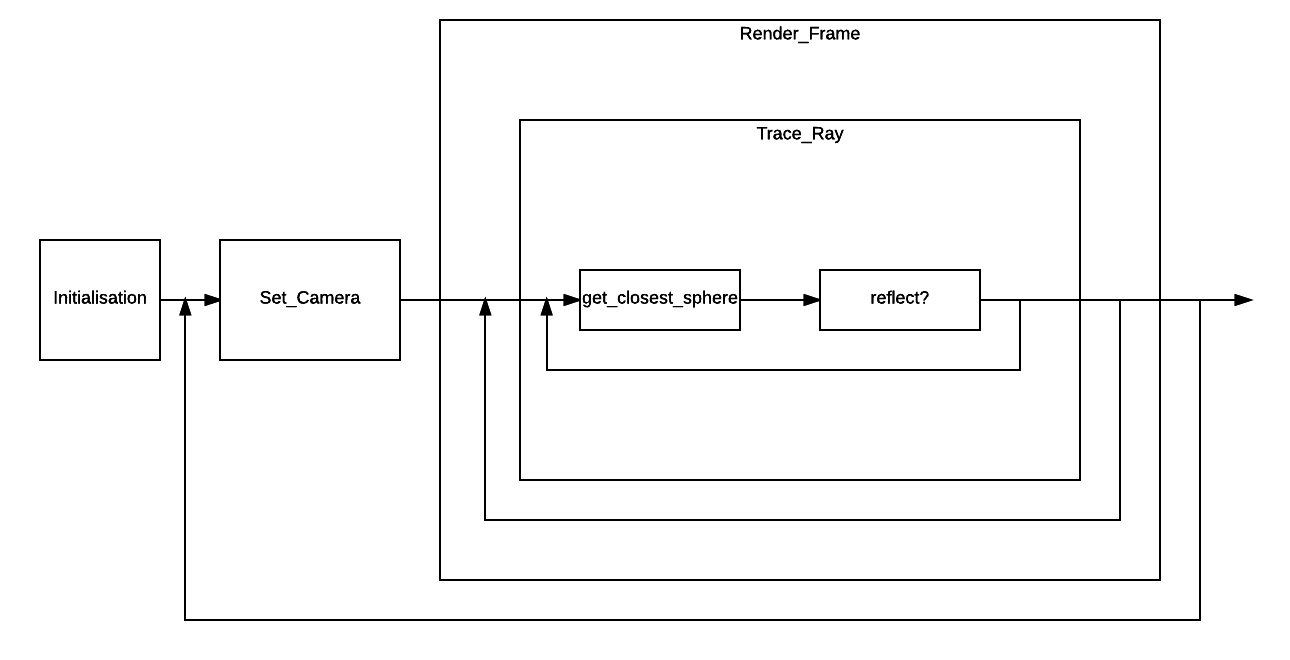
\includegraphics[width=\textwidth]{algo.png}
		\caption{Schematic of the algorithm}
	\label{fig1}
	\end{figure}
\end{frame}


\begin{frame} %%Eine Folie
	\frametitle{Functions} %%Folientitel
  	\begin{itemize}
		\item Initialisation: once in entire algorithm
		\item SetCamera: once every frame
		\item GetClosestSphere: up to REFLECT times per ray
		\item Reflect: up to REFLECT times per ray
	\end{itemize}
\end{frame}

\begin{frame} %%Eine Folie
	\frametitle{SW code structure} %%Folientitel
	getClosestSphere is a main function and contains a lot of loops\\
	$\quad$\\
	$\rightarrow$ Transition looped functions from SW to HW to achieve target speed
\end{frame}

\section{Optimization}


\begin{frame} %%Eine Folie
	\frametitle{Main Idea}
	\begin{itemize}
	\item automate entire render-frame function in one pipeline
	\item use memory mapped interface
	\item set pipeline parameters (mostly the spheres) at initialisation
	\end{itemize}
\end{frame}

\begin{frame} %%Eine Folie
	\frametitle{Calling the Pipeline} %%Folientitel
	\begin{itemize}
		\item Initialisation:\\
		each environment element has own address, write to it to update (no checks necessary)
		\item setCamera:\\
		each part of the camera has own address, write to it to update (read special address to see if write possible)
		\item startNewFrame:\\
		no special command necessary
		\item getResultingPixels:\\
		read special addresses
	\end{itemize}
\end{frame}

\begin{frame} %%Eine Folie
	\frametitle{Overview} %%Folientitel
	\begin{figure}[h]
		\centering
		\fbox{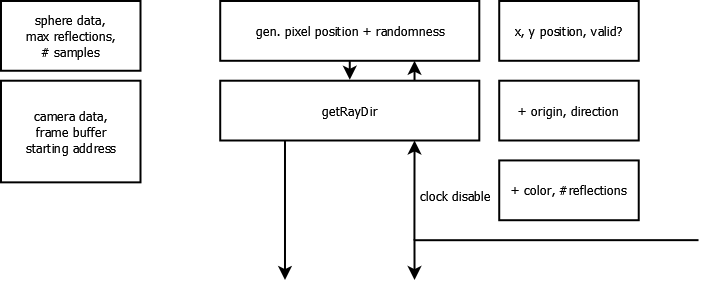
\includegraphics[width = 0.6\textwidth]{pics/frontend.png}}
		\caption{Pipepline 1}
	\end{figure}
\end{frame}
\begin{frame} %%Eine Folie
	\frametitle{Overview} %%Folientitel
	\begin{figure}[h]
		\centering
		\fbox{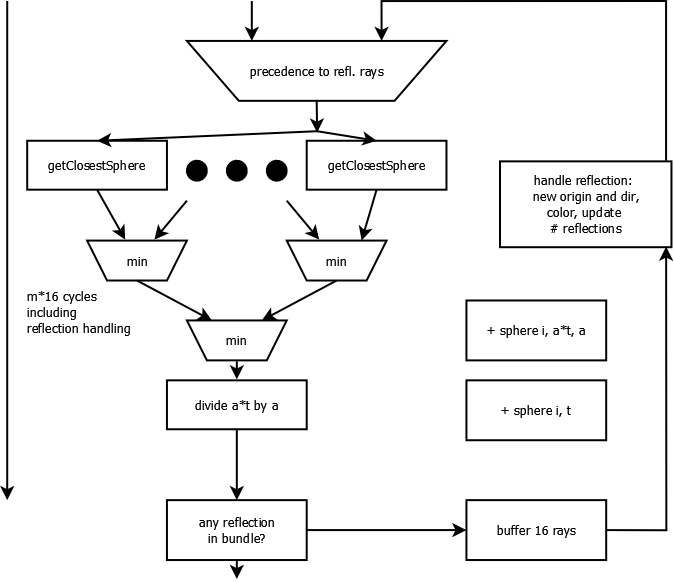
\includegraphics[width = 0.6\textwidth]{pics/middle.png}}
		\caption{Pipepline 2}
	\end{figure}
\end{frame}
\begin{frame} %%Eine Folie
	\frametitle{Overview} %%Folientitel
	\begin{figure}[h]
		\centering
		\fbox{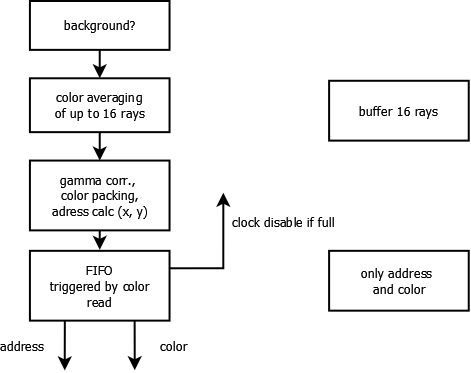
\includegraphics[width = 0.6\textwidth]{pics/backend.png}}
		\caption{Pipepline 3}
	\end{figure}
\end{frame}

\begin{frame} %%Eine Folie
	\frametitle{Calculating Initial Ray} %%Folientitel
	\begin{itemize}
		\item start with (0,0) as soon as all camera elements set
		\item add random offset within the pixel (in both directions)
		\item repeat number of samples times per pixel
		\item calculate the direction of the ray
	\end{itemize}
\end{frame}

\begin{frame} %%Eine Folie
	\frametitle{GetClosestSphere } %%Folientitel
	\begin{itemize}
		\item 8 parallel calculations for distance to spheres
		\item compare them at the end (7 comparators)
	\end{itemize}
	\textbf{if more than 8 spheres:}
	\begin{itemize}
		\item odd cycles spheres 1-8
		\item even cycles spheres 9-16
		\item additional comparison and stage
	\end{itemize}
\end{frame}

\begin{frame} %%Eine Folie
	\frametitle{Reflection} %%Folientitel
	\begin{itemize}
		\item start division (for reflection position)
		\item calculate colour change
		\item calculate reflection
		\item normalise by division result
		\item wait until all rays of one pixel are present (additional stages)
		\item reflect all rays of a pixel if one needs reflection (VALID bit)
	\end{itemize}
\end{frame}

\begin{frame}
\frametitle{Calculate Pixel} %%Folientitel
	\begin{itemize}
		\item average rays
		\item gamma correction
		\item colour packing
		\item sort by position of pixel
	\end{itemize}
\end{frame}


\section{Evaluation}
\begin{frame}
	\frametitle{Resources}
	\begin{itemize}
		\item 2x Random
		\item $\sim$ 90 Add/Sub
		\item $\sim$ 55 Multiplication
		\item $\sim$ 40 Square of Input
		\item 1 Divisions
		\item 2 Square Roots
		\item 1fifo
		\item $\sim$ 1000 registers
	\end{itemize}
\end{frame}

\begin{frame}
	\frametitle{Timing}
	\begin{itemize}
		
		\item \textbf{time lag for each ray} 40 + 96*reflects + samples
		\item \textbf{pipeline stages} 136 + samples
	\end{itemize}
	$\rightarrow$ with parameters reflects=5, samples=1, objects=5, a throughput of 1/5 pixles per second should be achievable
\end{frame}


\end{document}